\chapter*{Введение}                         % Заголовок
\addcontentsline{toc}{chapter}{Введение}    % Добавляем его в оглавление

\newcommand{\actuality}{}
\newcommand{\progress}{}
\newcommand{\aim}{{\textbf\aimTXT}}
\newcommand{\tasks}{\textbf{\tasksTXT}}
\newcommand{\novelty}{\textbf{\noveltyTXT}}
\newcommand{\influence}{\textbf{\influenceTXT}}
\newcommand{\methods}{\textbf{\methodsTXT}}
\newcommand{\defpositions}{\textbf{\defpositionsTXT}}
\newcommand{\reliability}{\textbf{\reliabilityTXT}}
\newcommand{\probation}{\textbf{\probationTXT}}
\newcommand{\contribution}{\textbf{\contributionTXT}}
\newcommand{\publications}{\textbf{\publicationsTXT}}


{\actuality}
Задачи термоупругости очень популярны в различных инженерных приложениях, так как температурные деформации могут существенным образом повлиять на функциональные свойста рассматриваемых объектов, вплоть до их полного выхода из строя. Особенно популярны такого рода задачи в аэрокосмической отрасли при моделировании поведения обшивок корпусов и двигателей летательных аппаратов \cite{Aerocosmos1, Aerocosmos2, Aerocosmos3}, так как они подвергаются очень высоким и в то же время неравномерным нагружениям \cite{Aerocosmos4, Aerocosmos5, Aerocosmos6, Aerocosmos7}. Помимо аэрокосмической отрасли такие задачи могут быть востребованы в строительстве, особенно в строительстве критической инфраструктуры, такой, например, как атомные электространции \cite{StroyMech1, StroyMech2}. Однако и гражданская инфраструктура подвергается анализу влияния таких разрушительных явлений как пожары \cite{StroyMech3, StroyMech4} или обычная циклическая смена сезона \cite{StroyMech5, StroyMech6} при воздействии которых конструкция не должна потерять устойчивость. В микроэлектронике эти задачи также не остаются без внимания \cite{MicroElectronic1, MicroElectronic2}, а учитывая возрастающее количество вычислительных мощностей и популярность носимой электроники возникают задачи об эффективном отводе тепловой энергии \cite{MicroElectronic3}.

Все перечисленные ранее и многие другие задачи объединяет потребность в создании новых материалов, которые будут отвечать соответствующим их использованию требованиям. На сегодняшний день, в некоторых отраслях требования к свойствам материалов становятся уже настолько высокими, что при их создании приходится учитывать структуру материала на микро- и наноуровне \cite{MaterialStructure1, MaterialStructure2, MaterialStructure3}, так как их свойства могут напрямую зависеть от молекулярной структуры. Такие материалы принято называть структурно-чувствительными материалами, а создание материалов с наперёд заданными свойствами на сегодняшний момент является одной из сложнейших, но вместе с этим крайне актуальной областью материаловедения \cite{Auxetics}.

Помимо проблемы создания структурно-чувствительных материалов многие исследователи также сталкиваются с проблемой моделирования их поведения. При рассмотрении наномасштабных структур пропадает возможность использовать гипотезу сплошности среды из-за чего классические модели механики сплошной среды не могут даже на качественном уровне передать все особенности их поведения. Преобладание таких эффектов как микровращения отдельных зёрен материала, микродислокации, различные дальнодействующие и многие другие масштабные эффекты могут быть смоделированы только при помощи новых математических моделей.

К счастью, на сегодняшний день существует большое количество моделей способных описать различные масштабные эффекты, однако, способы моделирования могут достаточно сильно различаться между собой при рассмотрении разных линейных размеров и временных отрезков. Таким образом возникают иерархии моделей способных качественно и количественно описать различные аспекты поведения материала на разных масштабах. Это в свою очередь приводит к идее многомасштабного моделирования \cite{Multiscale1}, где, например, некоторые характеристики материала можно вычислять при помощи моделей находящихся ниже по иерархии и передавать полученные в расчётах параметры в вышестоящие модели.

Для механики твёрдого тела одна из возможных иерархий моделей проиллюстрирована на рис. \ref{fig:ModelsHierarchy}. Согласно такому представлению, модели использующие аппарат квантовой механики \cite{QuantumModelling1, QuantumModelling2} находятся на первой ступени иерархии, а их применение ограничено масштабами сопоставимыми с ядрами атомов и их молекулярных соединений, то есть в диапазоне от нескольких ангстрем до нескольких нанометров. На второй ступене иерархии находятся модели молекулярной динамики \cite{MD1, MD2, MD3, MD4}, такие модели могут описывать поведение сложных соединений, например, больших полимерных молекул и прочих наномасштабных объектов, размеры которых не превосходят нескольких десятков нанометров. На третьей ступене располагаются статистические модели, в частности модели в основе которых лежит метод Монте-Карло \cite{MonteCarlo1, MonteCarlo2}. В таких моделях расчёты проводятся многократно, а структура рассматриваемого объекта генерируется случайным образом по особым правилам после чего полученные таким способом результаты осредняют или вычисляют на их основе вероятностные характеристики материала. И на последней --- четвёртой ступени иерархии стоят континуальные модели, в частности модели механики сплошной среды \cite{MSS}. Такие модели оперируют гипотезой сплошностью среды и абсолютности времени, то есть не учитывают дискретность рассматриваемого вещества.

\begin{figure}[ht]
    \centerfloat{
        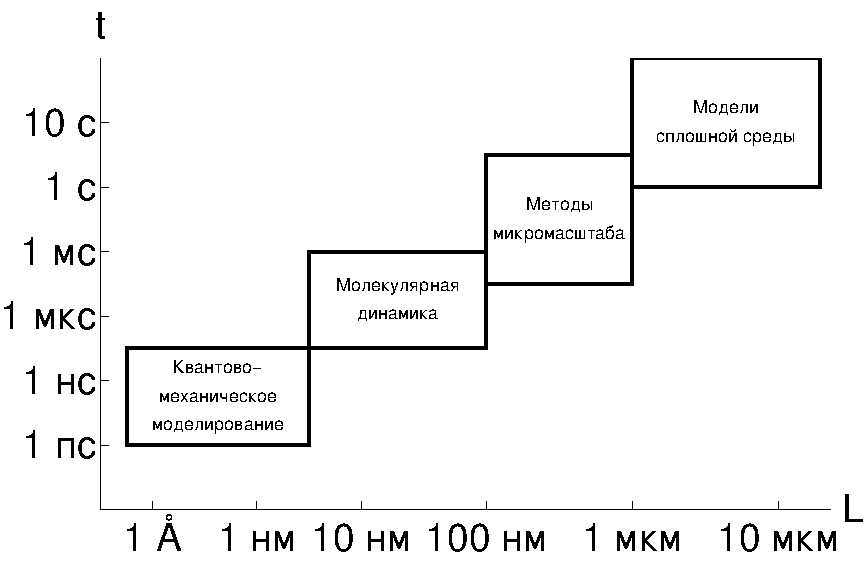
\includegraphics[width=0.85\textwidth]{pics/ModelsHierarchy.pdf}
    }
    \caption{Иерархия моделей.}\label{fig:ModelsHierarchy}
\end{figure}

Однако, несмотря на то, что модели молекулярной динамики и статистические модели находятся на более низких ступенях иерархии, чем модели сплошной среды, анализ объектов при помощи этих моделей без численных экспериментов крайне ограничен \cite{MDExperiment}. Поэтому с середины XX века набирают популярность модели обобщённой механики сплошной среды, которые распространяют применение моделей высшего уровня на области применения моделей низшего уровня. Одна из первых таких моделей была предложена в работе братьев Эжен и Франсуа Коссера \cite{Cosserat}, где помимо трансляционных степеней свободы также учитывались и вращательные компоненты движения, которые связаны с трансляционными рядом соотношений из-за чего тензор напряжений становится нессиметричным. Позже, спустя пол века, эта теория была связана с теорией дислокаций в работе V.~G{\"u}nther \cite{CosseratAndDislocation} и дополнена законом сохранения микроинерции в работе A.C.~Eringen \cite{Eringen2, Eringen3} в связи с чем теорию начали называть микрополярной теорией упругости. Также к работам связанным с исследованием микрополярной теории упругости можно отнести работы R.D.~Mindlin \cite{Mindlin1, Mindlin2, Mindlin3}, и работы D.B.~Bogy \cite{Bogy} и Y.C.~Hsu \cite{Hsu}, в которых авторы рассматривали применение этой теории к задачам с концентраторами возникающим в углах и отверстиях соответсвенно. В это же время теория приобрела своё развитие в работах советских учёных Э.Л.~Аэро и Е.В.~Кувшинского \cite{Aero1,Aero2}, а также была рассмотрена в работах Н.Ф.~Морозова \cite{Morozov} и Г.Н. Савина \cite{Savin}.

Дальнейшее развитие микрополярной теории упругости привело к появлению микроморфных моделей \cite{Eringen4, Micromorph1, Micromorph2}, в которые помимо вращательных компонент движения могут быть включены дополнительные переменные связанные с деформацией материала, при этом микрополярная теория упругости ялвяется лишь частным случаем микроморфных моделей. К сожалению, использование таких моделей сопряжено с трудностью определения материальных коэффициентов, которых в такого рода моделях становится достаточно много.

Список рассмотренных моментных моделей, а также авторов, которые занимались их развитием и исследованием далеко не исчерпывающий, однако, стоит также уделить внимание другому классу моделей обобщённой механики сплошной среды учитывающих дальнодействующие эффекты. Это градиентные и нелокальные модели, которые также получили своё развитие в 60-х годах XX века. Первые модели градиентной теории упругости были сформулированы в работах Toupin~R.A. \cite{Toupin} и Mindlin~R.D. \cite{Mindlin4, Mindlin5}, которые сейчас в литературе принято называть моделями Миндлина --- Тупина \cite{ToupinMindlin1, ToupinMindlin2, ToupinMindlin3}. Позже в работе G.~Ahmadi и K.~Firoozbakhsh \cite{GradientThermoelasticity} эти модели получили связь с температурными деформациями. Но как и микроморфные модели градиентные модели обладают тем же недостатком --- большое количество материальных констант, которые необходимо определить, поэтому в 90-х годах XX века в работах E.C.~Aifantis и его соавторов \cite{Aifantis1, Aifantis2} была рассмотренна упрощёная модель градиентной теории упругости, в которой напряжения зависят от деформации и её второго градиента, а также введён всего один дополнительный материальный параметр внутренней длины.

Нелокальные модели в отличие от градиентных оперируют интегральными выражениями типа свёртки. Впервые описание таких моделей было представлено в работе E.~Kr{\"o}ner \cite{Kroner}, где рассматривались упругие среды с дальнодействующими силами сцепления. Модели нелокальной упругости в термодинамическом контексте были рассмотрены в работах D.G.B.~Edelen, A.E.~Green и N.~Laws \cite{Edelen1, Edelen2}, позже к работе присоединился и A.C.~Eringen \cite{Eringen5, Eringen6}. Исследование условий обеспечивающих существование фундаментнальных решений было проведено в работе D. Rogula \cite{Rogula1982}. Вопросы, связанные с существованием и единственностью решения нелокальной начально-краевых задач упругости были рассмотрены в работах S.B.~Altan \cite{Altan1, Altan2}, а также для задач нелокальной термоупругости \cite{Altan3, Altan4}. В дальнейшем A.C.~Eringen представит работу, в которой описан единый подход к построению нелокальных теорий для упругих тел в работе \cite{Eringen1}, в связи с чем в литературе нелокальные модели часто называют моделями Эрингена \cite{BondaryLayer, Tuna, Rahmani}.

Связь градиентной модели Айфантиса и нелокальной \cite{Aifantis3, Gao}.

Текущая работа посвящена исследованию нелокальных моделей, а точнее даже их модификации с добавлением регуляризационного слагаемого относящегося к классической или локальной теории. Такой подход был предложен в работе Polizzoto \cite{Polizzotto1}.

\cite{SaintVenant}.

Поиск решений интегро-дифференциальных уравнений представляет из себя достаточно сложную задачу. В этом случае необходимо прибегать к использованию различных численных методов, специально адаптированных под данный класс уравнений. В этом направлении есть уже достаточно большое количество работ, предлагающие использовать различные методы решения. Наиболее общим и популярным является метод конечных элементов (FEM), который применительно к данному классу уравнений иногда ещё называют методом нелокальных конечных элементов (NL-FEM) \cite{Polizzotto2, Pisano1}. Однако его использование сопряжёно с большой вычислительной сложностью, поэтому некоторые ииследователи прибегают к возможностям интегральных преобразований откуда был получен метод на основе быстрого преобразования Гаусса (FEMFGT) \cite{FastGaussTransform}. К сожалению, использование этого метода сопряжено с рядом трудностей, так как для его применения необходима достаточно подробная сетка, чтобы избежать возможных осциляций решения, также сложность вызывает контроль точности получаемых решений. Помимо сеточных методов большой популярностью пользуются и бессеточные подходы на основе радиальных базисных функций \cite{RadialBasis}, безэлементный метод Галёркина (EFG) и метод конечных точек (FPM) \cite{MeshFree}. Также были предложены подходы с использованием пограничного слоя \cite{BondaryLayer} и на основе полиномов Чебышева \cite{ChebPolynom}.

В рамках этой работы было принято решение остановиться на методе конечных элементов, так как этот метод достаточно хорошо изучен и его относительно легко реализовать и модифицировать под рассматриваемый класс уравнений. Также этим методом легко решать задачи на областях со сложной геометрической формой, а большое количество редакторов и генераторов сеток упрощает процесс моделирования. Реализация данного метода включена в программный комплекс NonLocFEM, структуру которого мы рассмотрим в третьей главе диссертации.

%\ifsynopsis
%Этот абзац появляется только в~автореферате.
%\else
%Этот абзац появляется только в~диссертации.
%\fi

% {\progress}
% Этот раздел должен быть отдельным структурным элементом по
% ГОСТ, но он, как правило, включается в описание актуальности
% темы. Нужен он отдельным структурынм элемементом или нет ---
% смотрите другие диссертации вашего совета, скорее всего не нужен.

{\aim}
исследования является изучение особенностей рассматриваемых моделей термоупругости, а также сравнение решений полученных при их использовании с решениями полученными при использовании классических моделей механики сплошной среды.

Для достижения поставленной цели потребовалось решить {\tasks}:
\begin{enumerate}[beginpenalty=10000] % https://tex.stackexchange.com/a/476052/104425
  \item Разработка определяющих соотношений модели термоупругости нелокальной среды в интегро-дифференциальной форме..
  \item Разработка алгоритмов численного решения с их последующей оптизацией для более эффективного использования на многопроцессорных вычислительных машинах.
  \item Реализация полученных алгоритмов в виде программного комплекса.
  \item Исследование поведения модели на примере решения определённого ряда задач с известными решениями в классической постановке, сравнение получившихся решений и определение закономерностей.
\end{enumerate}


{\novelty}
\begin{enumerate}[beginpenalty=10000] % https://tex.stackexchange.com/a/476052/104425
  \item Разработаны эффективные методы решения на основе метода конечных элементов с обобщением на интегро-дифференциальные уравнения, которые обладают хорошей масштабируемостью и предназначены для вычислений на многопроцессорных вычислительных машинах с общей и распределённой памятью.
  \item Разработан программный комплекс NonLocFEM, в котором реализованы все представленные в работе алгоритмы и методы для моделирования поведения структруно-чувствительных материалов.
  \item Проведено качественное сравнение между результатами полученными с использованием классической и нелокальной теориями, которые свидетельствуют о снижении роли концентраторов в распределениях полей напряжений и плотности теплового потока.
  \item Исследованы границы спектров собственных чисел матриц и установлены связи между спектрами матриц ассемблированных в классической и нелокальной постановках.
\end{enumerate}

{\influence}
моделей рассмотренных в диссертации состоит в возможности описания поведения термомеханических состояний структурно-чувствительных материалов, параметры модели очевидным образом влияют на решения, что позволяет тонко настраивать модель при исследованиях. Разработанный программный комплекс дополняет рассматриваемую модель, позволяет проводить расчёты на произвольных областях со всеми рассматриваемыми в моделе параметрами, а благодаря открытому исходному код и модульной структуре существует возможность без труда вносить в него изменения и добавлять новые типы расчётов при модификации математической модели.

{\methods}
В диссертации используются как классические принципы механики деформируемого твёрдого тела, так и новые относящиеся к нелокальной теории термоупругости, а также численные методы в основе которых лежит метод конечных элементов.

{\defpositions}
\begin{enumerate}[beginpenalty=10000] % https://tex.stackexchange.com/a/476052/104425
 	\item Модель нелокальной термоупругости позволяющая описать процессы теплопроводности и напряжённо-деформированного состояния в структурно-чувствительных материалах.
	\item Численный алгоритм решения на основе метода конечных элементов, адапатированный под многопроцессорные вычислительные системы.
	\item Программный комплекс NonLocFEM, в рамках которого реализованы все рассматриваемые в работе методы решений.
\end{enumerate}

{\reliability} гарантирует строгость используемого математического аппарата, сравнение расчётов с известными теоретическими результатами и аналитическими решениям, а также результатами, полученными ранее другими авторами.


{\probation}
проводилась в обсуждениях на следующих конференциях:
\begin{enumerate}
	\item Международная научно-техническая конференция <<Актуальные проблемы прикладной математики, информатикии и механики>> (Воронеж, 2019, 2021);
	\item Международная конференция <<International Conference of Numerical Analysis and Applied Mathematics>> (Родос, Греция, 2021);
	\item Международная научная конференция <<Фундаментальные и Прикладные Задачи Механики>> (Москва, 2021);
	\item Всероссийская конференция по численным методам решения задач теории упругости и пластичности (Красноярск, 2023);
	\item Математическое моделирование, численные методы и инженерное программное обеспечение (Москва, 2023).
\end{enumerate}

{\contribution}
Все исследования, представленные в диссертационной работе, а также разработка программного комплекса выполнены лично соискателем в процессе научной деятельности. Из совместных публикаций в диссертацию включен лишь тот материал, который принадлежит соискателю, заимствованный материал обозначен в работе ссылками.

\ifnumequal{\value{bibliosel}}{0}
{%%% Встроенная реализация с загрузкой файла через движок bibtex8. (При желании, внутри можно использовать обычные ссылки, наподобие `\cite{vakbib1,vakbib2}`).
    {\publications} Основные результаты по теме диссертации изложены
    в~XX~печатных изданиях,
    X из которых изданы в журналах, рекомендованных ВАК,
    X "--- в тезисах докладов.
}%
{%%% Реализация пакетом biblatex через движок biber
    \begin{refsection}[bl-author, bl-registered]
        % Это refsection=1.
        % Процитированные здесь работы:
        %  * подсчитываются, для автоматического составления фразы "Основные результаты ..."
        %  * попадают в авторскую библиографию, при usefootcite==0 и стиле `\insertbiblioauthor` или `\insertbiblioauthorgrouped`
        %  * нумеруются там в зависимости от порядка команд `\printbibliography` в этом разделе.
        %  * при использовании `\insertbiblioauthorgrouped`, порядок команд `\printbibliography` в нём должен быть тем же (см. biblio/biblatex.tex)
        %
        % Невидимый библиографический список для подсчёта количества публикаций:
        \printbibliography[heading=nobibheading, section=1, env=countauthorvak,          keyword=biblioauthorvak]%
        \printbibliography[heading=nobibheading, section=1, env=countauthorwos,          keyword=biblioauthorwos]%
        \printbibliography[heading=nobibheading, section=1, env=countauthorscopus,       keyword=biblioauthorscopus]%
        \printbibliography[heading=nobibheading, section=1, env=countauthorconf,         keyword=biblioauthorconf]%
        \printbibliography[heading=nobibheading, section=1, env=countauthorother,        keyword=biblioauthorother]%
        \printbibliography[heading=nobibheading, section=1, env=countregistered,         keyword=biblioregistered]%
        \printbibliography[heading=nobibheading, section=1, env=countauthorpatent,       keyword=biblioauthorpatent]%
        \printbibliography[heading=nobibheading, section=1, env=countauthorprogram,      keyword=biblioauthorprogram]%
        \printbibliography[heading=nobibheading, section=1, env=countauthor,             keyword=biblioauthor]%
        \printbibliography[heading=nobibheading, section=1, env=countauthorvakscopuswos, filter=vakscopuswos]%
        \printbibliography[heading=nobibheading, section=1, env=countauthorscopuswos,    filter=scopuswos]%
        %
        \nocite{*}%
        %
        {\publications} Основные результаты по теме диссертации изложены в~\arabic{citeauthor}~печатных изданиях,
        \arabic{citeauthorvak} из которых изданы в журналах, рекомендованных ВАК\sloppy%
        \ifnum \value{citeauthorscopuswos}>0%
            , \arabic{citeauthorscopuswos} "--- в~периодических научных журналах, индексируемых Web of~Science и Scopus\sloppy%
        \fi%
        \ifnum \value{citeauthorconf}>0%
            , \arabic{citeauthorconf} "--- в~тезисах докладов.
        \else%
            .
        \fi%
        \ifnum \value{citeregistered}=1%
            \ifnum \value{citeauthorpatent}=1%
                Зарегистрирован \arabic{citeauthorpatent} патент.
            \fi%
            \ifnum \value{citeauthorprogram}=1%
                Зарегистрирована \arabic{citeauthorprogram} программа для ЭВМ.
            \fi%
        \fi%
        \ifnum \value{citeregistered}>1%
            Зарегистрированы\ %
            \ifnum \value{citeauthorpatent}>0%
            \formbytotal{citeauthorpatent}{патент}{}{а}{}\sloppy%
            \ifnum \value{citeauthorprogram}=0 . \else \ и~\fi%
            \fi%
            \ifnum \value{citeauthorprogram}>0%
            \formbytotal{citeauthorprogram}{программ}{а}{ы}{} для ЭВМ.
            \fi%
        \fi%
        % К публикациям, в которых излагаются основные научные результаты диссертации на соискание учёной
        % степени, в рецензируемых изданиях приравниваются патенты на изобретения, патенты (свидетельства) на
        % полезную модель, патенты на промышленный образец, патенты на селекционные достижения, свидетельства
        % на программу для электронных вычислительных машин, базу данных, топологию интегральных микросхем,
        % зарегистрированные в установленном порядке.(в ред. Постановления Правительства РФ от 21.04.2016 N 335)
    \end{refsection}%
    \begin{refsection}[bl-author, bl-registered]
        % Это refsection=2.
        % Процитированные здесь работы:
        %  * попадают в авторскую библиографию, при usefootcite==0 и стиле `\insertbiblioauthorimportant`.
        %  * ни на что не влияют в противном случае
        \nocite{vakbib2}%vak
        \nocite{patbib1}%patent
        \nocite{progbib1}%program
        \nocite{bib1}%other
        \nocite{confbib1}%conf
    \end{refsection}%
        %
        % Всё, что вне этих двух refsection, это refsection=0,
        %  * для диссертации - это нормальные ссылки, попадающие в обычную библиографию
        %  * для автореферата:
        %     * при usefootcite==0, ссылка корректно сработает только для источника из `external.bib`. Для своих работ --- напечатает "[0]" (и даже Warning не вылезет).
        %     * при usefootcite==1, ссылка сработает нормально. В авторской библиографии будут только процитированные в refsection=0 работы.
}

%При использовании пакета \verb!biblatex! будут подсчитаны все работы, добавленные
%в файл \verb!biblio/author.bib!. Для правильного подсчёта работ в~различных
%системах цитирования требуется использовать поля:
%\begin{itemize}
%        \item \texttt{authorvak} если публикация индексирована ВАК,
%        \item \texttt{authorscopus} если публикация индексирована Scopus,
%        \item \texttt{authorwos} если публикация индексирована Web of Science,
%        \item \texttt{authorconf} для докладов конференций,
%        \item \texttt{authorpatent} для патентов,
%        \item \texttt{authorprogram} для зарегистрированных программ для ЭВМ,
%        \item \texttt{authorother} для других публикаций.
%\end{itemize}
%Для подсчёта используются счётчики:
%\begin{itemize}
%        \item \texttt{citeauthorvak} для работ, индексируемых ВАК,
%        \item \texttt{citeauthorscopus} для работ, индексируемых Scopus,
%        \item \texttt{citeauthorwos} для работ, индексируемых Web of Science,
%        \item \texttt{citeauthorvakscopuswos} для работ, индексируемых одной из трёх баз,
%        \item \texttt{citeauthorscopuswos} для работ, индексируемых Scopus или Web of~Science,
%        \item \texttt{citeauthorconf} для докладов на конференциях,
%        \item \texttt{citeauthorother} для остальных работ,
%        \item \texttt{citeauthorpatent} для патентов,
%        \item \texttt{citeauthorprogram} для зарегистрированных программ для ЭВМ,
%        \item \texttt{citeauthor} для суммарного количества работ.
%\end{itemize}
% Счётчик \texttt{citeexternal} используется для подсчёта процитированных публикаций;
% \texttt{citeregistered} "--- для подсчёта суммарного количества патентов и программ для ЭВМ.

%Для добавления в список публикаций автора работ, которые не были процитированы в
%автореферате, требуется их~перечислить с использованием команды \verb!\nocite! в
%\verb!Synopsis/content.tex!.
 % Характеристика работы по структуре во введении и в автореферате не отличается (ГОСТ Р 7.0.11, пункты 5.3.1 и 9.2.1), потому её загружаем из одного и того же внешнего файла, предварительно задав форму выделения некоторым параметрам

\textbf{Объем и структура работы.} Диссертация состоит из~введения,
\formbytotal{totalchapter}{глав}{ы}{}{} и
заключения и
\formbytotal{totalappendix}{приложен}{ия}{ий}{}.
%% на случай ошибок оставляю исходный кусок на месте, закомментированным
%Полный объём диссертации составляет  \ref*{TotPages}~страницу
%с~\totalfigures{}~рисунками и~\totaltables{}~таблицами. Список литературы
%содержит \total{citenum}~наименований.
%
Полный объём диссертации составляет
\formbytotal{TotPages}{страниц}{у}{ы}{}, включая
\formbytotal{totalcount@figure}{рисун}{ок}{ка}{ков} и
\formbytotal{totalcount@table}{таблиц}{у}{ы}{}.
Список литературы содержит
\formbytotal{citenum}{наименован}{ие}{ия}{ий}.
